\documentclass{article}

\usepackage[utf8]{inputenc}
\usepackage{enumitem}
\usepackage{amsmath}
\usepackage{amsthm}
\usepackage{amssymb}
\usepackage{graphicx}
\usepackage{tikz}
\usepackage[normalem]{ulem}

\newcommand{\mname}[1]{\mbox{\sf #1}}
\newcommand{\pnote}[1]{{\langle \text{#1} \rangle}}

\newcommand{\GETS}{:=}

%% Highlight, strike-out
\newcommand{\key}[1]{\underline{\smash{#1}}}
\newcommand{\pkey}[1]{\dashuline{\smash{#1}}}

%% SQL
\newcommand{\SQL}[1]{\texttt{#1}}
\newcommand{\SQLK}[1]{\texttt{\bf #1}}
\newcommand{\SQLCOMMENT}{\texttt{-}\texttt{-} }

%% RA
\newcommand{\rename}{\rho}
\newcommand{\select}{\sigma}
\newcommand{\join}{\times}
\newcommand{\rel}[1]{\text{#1}}
\newcommand{\attr}[1]{\text{#1}}
\newcommand{\ra}[2]{\rel{#1}.\attr{#2}}
\newcommand{\project}{\pi}
\newcommand{\product}{\times}
\newcommand{\union}{\cup}
\newcommand{\intersect}{\cap}
\newcommand{\difference}{\setminus}
\newcommand{\goesto}[2]{#1 \mapsto #2}
\newcommand{\njoin}{\Join}
\newcommand{\dedup}{\delta}
\newcommand{\group}{\gamma}

\title{Assignment 4: The Relational Algebra}
\author{Hien Tu - tun1}
\date{\today}

\begin{document}

\maketitle

\textbf{The requested queries}
\begin{enumerate}
  \item $\select_{\attr{startdate } < \attr{ enddate}}(\rel{event})$ \\
  \item $\project_{\ra{U}{uid}, \ra{E}{eid}}
          (\rename_{\rel{U}}(\rel{user}) \Join_{\ra{U}{postcode } = \ra{ E}{postcode }}
          \rename_{\rel{E}}(\rel{event}))$ \\
  \item $X \GETS
          \rename_{\rel{E}}(\rel{event}) \Join_{\ra{E}{eid } = \ra{ EnoRv}{eid}}
          \rename_{\rel{EnoRv}}
            (\project_{\attr{eid}}(\rel{event}) \difference
            \project_{\attr{event}}(\rel{review}))$ \\
        $\project_{\ra{E}{eid}, \ra{E}{title}, \ra{E}{description},
          \ra{E}{startdate}, \ra{E}{enddate}, \ra{E}{organizer},
          \ra{E}{postcode}}(X)$ \\
  \item Select events with at least 3 keywords: \\
        $X \GETS \rename_{\rel{K}_1}(\attr{keyword}) \product
                  \rename_{\rel{K}_2}(\attr{keyword}) \product
                  \rename_{\rel{K}_3}(\attr{keyword})$ \\
        $Y \GETS \select_{K_1.\attr{word } \neq K_2.\attr{ word } \land
                          K_1.\attr{word } \neq K_3.\attr{ word } \land
                          K_2.\attr{word } \neq K_3.\attr{ word }}(X)$ \\
        $Z \GETS \select_{K_1.\attr{event } = K_2.\attr{event } \land
                          K_1.\attr{event } = K_3.\attr{event }}(Y)$ \\ \\
        Select events with at least 2 keywords: \\
        $A \GETS \rename_{\rel{K}_4}(\attr{keyword}) \product
                  \rename_{\rel{K}_4}(\attr{keyword})$ \\
        $B \GETS \select_{K_4.\attr{word } \neq K_5.\attr{word}}(A)$ \\
        $C \GETS \select_{K_4.\attr{event } = K_5.\attr{event}}(B)$ \\ \\
        Select events with exactly 3 keywords: \\
        $\project_{K_4.event}(C) \difference \project_{K_1.event}(Z)$ \\
  \item
    \begin{enumerate}
      \item $X \GETS \rename_{R_1}(\rel{review}) \product
                      \rename_{R_2}(\rel{review})$ \\ \\
            Keep reviews from $R_1$ that are not from latest date: \\
            $Y \GETS \select_{R_1.\attr{reviewdate } < R_2.\attr{reviewdate }
                              \land R_1.\attr{user } = R_2.\attr{user }}(X)$ \\ \\
            Select user id and event id for which the user wrote a review most
            recently: \\
            $Z \GETS
              \project_{\attr{user}, \attr{event}}(\rel{review}) \difference
              \project_{R_1.\attr{user}, R_1.\attr{event}}(Y)$ \\
      \item $A \GETS \rename_{R_1}(\rel{review}) \product
                      \rename_{R_2}(\rel{review}) \product
                      \rename_{E_1}(\rel{event}) \product
                      \rename_{E_2}(\rel{event})$ \\
            $B \GETS \select_{R_1.\attr{user } = R_2.\attr{user } \land
                              R_1.\attr{event } = E_1.\attr{eid } \land
                              R_2.\attr{event } = E_2.\attr{eid }}(A)$ \\ \\
            Select reviews whose $E_1.\attr{enddate}$ are not from the latest: \\
            $C \GETS \select_{E_1.\attr{enddate} < E_2.\attr{enddate}(B)}$ \\ \\
            Select user id and event id of the most-recent event (according to
            enddate) for which the user wrote a review: \\
            $D \GETS \project_{R_1.\attr{user}, E_1.\attr{eid}}(B \difference C)$ \\
      \item $\project_{\ra{LR}{user}, \ra{LR}{lreview}, \ra{LE}{levent}}
              (\rename_{\rel{LR}(\rel{user}, \rel{lreview})}(Z)
                \njoin_{\ra{LR}{user } = \ra{LE}{user}}
                \rename_{\rel{LE}(\rel{user}, \rel{levent})}(D))$ \\
    \end{enumerate}

\end{enumerate}


\textbf{Effiency of queries}
\begin{enumerate}
  \setcounter{enumi}{6}
  \item \ \\
    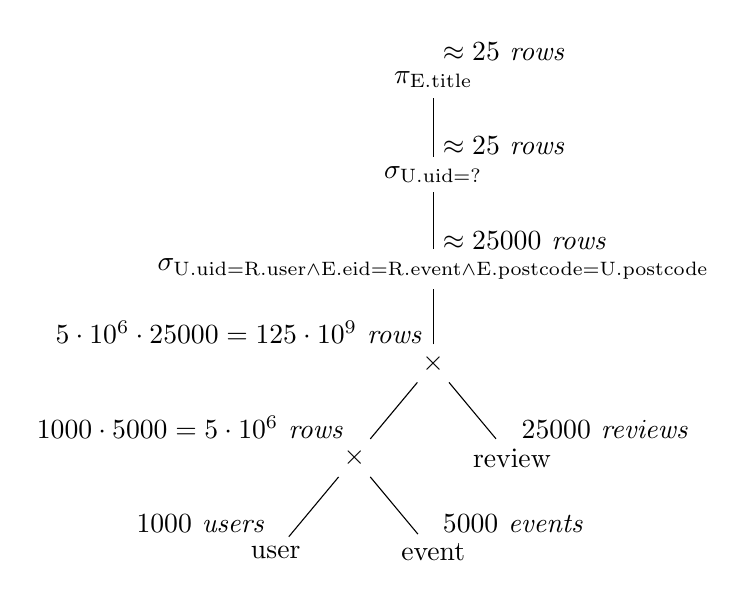
\begin{tikzpicture}[yscale=1.2]
      \node (p) at (0, 0) {$\project_{\ra{E}{title}}$};
      \node[above right] at (p) {\strut{}\emph{$\approx 25$ rows}};
      \node (su) at (0, -1) {$\select_{\ra{U}{uid} = ?}$} edge (p);
      \node[above right] at (su) {\strut{}\emph{$\approx 25$ rows}};
      \node (ss) at (0, -2) {$\select_{\ra{U}{uid} = \ra{R}{user} \land \ra{E}{eid} = \ra{R}{event} \land \ra{E}{postcode} = \ra{U}{postcode}}$} edge (su);
      \node[above right] at (ss) {\strut{}\emph{$\approx 25000$ rows}};
      \node (uer) at (0, -3) {$\product$} edge (ss);
      \node[above left] at (uer) {\strut{}\emph{$5 \cdot 10^6 \cdot 25000 = 125 \cdot 10^9$ rows}};
      \node (rv) at (1, -4) {$\rel{review}$} edge (uer);
      \node[above right] at (rv) {\strut{}\emph{$25000$ reviews}};
      \node (ue) at (-1, -4) {$\product$} edge (uer);
      \node[above left] at (ue) {\strut{}\emph{$1000 \cdot 5000 = 5 \cdot 10^6$ rows}};
      \node (u) at (-2, -5) {$\rel{user}$} edge (ue);
      \node[above left] at (u) {\strut{}\emph{$1000$ users}};
      \node (e) at (0, -5) {$\rel{event}$} edge (ue);
      \node[above right] at (e) {\strut{}\emph{$5000$ events}};
    \end{tikzpicture} \\

  \item \ \\
    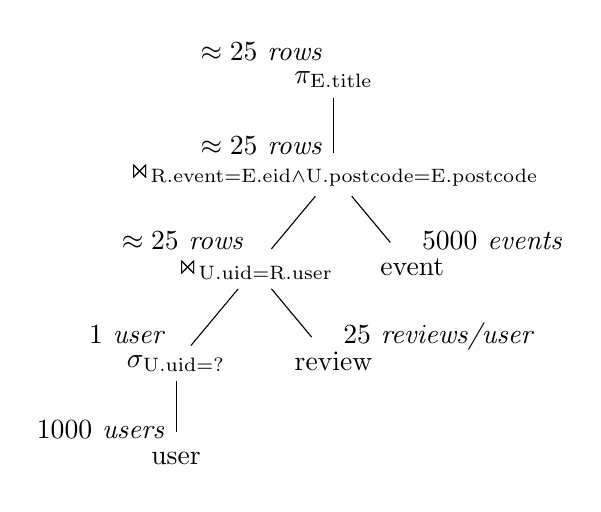
\begin{tikzpicture}[yscale=1.2]
      \node (s) at (-1, 0) {\strut{}user};
      \node[above left] at (s) {\strut{}\emph{$1000$ users}};
      \node (ss) at (-1, 1) {$\select_{\ra{U}{uid} = ?}$} edge (s);
      \node[above left] at (ss) {\strut{}\emph{$1$ user}};
      \node (ei) at (1, 1) {\strut{}review};
      \node[above right] at (ei) {\strut{}\emph{$25$ reviews/user}};
      \node (ssei) at (0, 2) {$\njoin_{\ra{U}{uid} = \ra{R}{user}}$} edge (ss) edge (ei);
      \node[above left] at (ssei) {\strut{}\emph{$\approx 25$ rows}};
      \node (c) at (2, 2) {\strut{}event};
      \node[above right] at (c) {\strut{}\emph{$5000$ events}};
      \node (cssei) at (1, 3) {$\njoin_{\ra{R}{event} = \ra{E}{eid} \land \ra{U}{postcode} = \ra{E}{postcode}}$} edge (ssei) edge (c);
      \node[above left] at (cssei) {\strut{}\emph{$\approx 25$ rows}};
      \node (pr) at (1, 4) {$\project_{\ra{E}{title}}$} edge (cssei);
      \node[above left] at (pr) {\strut{}\emph{$\approx 25$ rows}};
    \end{tikzpicture}

    From the query execution plan in question 7, we can see that the result of
    the cross product of the 3 tables, \emph{user}, \emph{review} and
    \emph{event} would have $125 \cdot 10^9$ rows, which is enormous. We can
    reduce this significantly by first selecting the row from the table
    \emph{user} where the \emph{uid} is equal to the required user id (in this
    case, denoted as $?$). This will result in only 1 rows since each \emph{uid}
    is unique. After that, we will join the result with the \emph{review}.
    Although the table \emph{review} has 25000 rows, each user only has 25
    reviews and since we have selected only 1 user, the result of this join
    would have approximately 25 rows. Then, we join this result with the table
    \emph{event}. Again, although the table \emph{event} has 5000 rows, since
    the previous result only has approximately 25 rows, there are only
    approximately 25 different event id. Thus, the result of this join only
    contains approximately 25 rows. Projecting just takes the specified column
    so the result of the whole query execution plan would have approximately 25
    rows. This execution plan is good since the returned table in each
    intermediate step is significantly small.

  \item The answer for question 9 is given in the answer for question 8.

  \item
    \begin{quote}
      \SQL{\SQLK{SELECT} \SQLK{DISTINCT} E.title\\
      \SQLK{FROM} user U, event E, review R\\
      \SQLK{WHERE} U.uid = $?$ \SQLK{AND}\\
      \phantom{\SQLK{WHERE}} R.user = U.uid \SQLK{AND}\\
      \phantom{\SQLK{WHERE}} R.event = E.eid \SQLK{AND}\\
      \phantom{\SQLK{WHERE}} U.postcode = E.postcode;} \\
    \end{quote}

  \item The given SQL query can be simplified to
    \begin{quote}
      \SQL{\SQLK{SELECT} \SQLK{DISTINCT} K.word\\
      \SQLK{FROM} user U, review Rv, keyword K, event E, region Rg\\
      \SQLK{WHERE} U.uid = $?_1$ \SQLK{AND}\\
      \phantom{\SQLK{WHERE}} Rv.user = U.uid \SQLK{AND}\\
      \phantom{\SQLK{WHERE}} Rv.event = K.eid \SQLK{AND}\\
      \phantom{\SQLK{WHERE}} E.postcode = Rg.postcode \SQLK{AND}\\
      \phantom{\SQLK{WHERE}} Rg.name = $?_2$ \SQLK{AND} \\
      \phantom{\SQLK{WHERE}} K.event = E.eid;}
    \end{quote}

    Thus, the relational algebra for the SQL query is \\
    $X \GETS \rename_{\rel{U}}(\rel{user}) \product
              \rename_{\rel{Rv}}(\rel{review}) \product
              \rename_{\rel{K}}(\rel{keyword}) \product
              \rename_{\rel{E}}(\rel{event}) \product
              \rename_{\rel{Rg}}(\rel{region})$ \\
    $Y \GETS \select_{\ra{U}{uid} = ?_1 \land
                        \ra{Rv}{user} = \ra{U}{uid} \land
                        \ra{Rv}{event} = \ra{K}{event} \land
                        \ra{E}{postcode} = \ra{Rg}{postcode} \land
                        \ra{Rg}{name} = ?_2 \land
                        \ra{K}{event} = \ra{E}{eid}}(X)$ \\
    $\project_{\ra{K}{word}}(Y)$ \\

  \item \ \\
    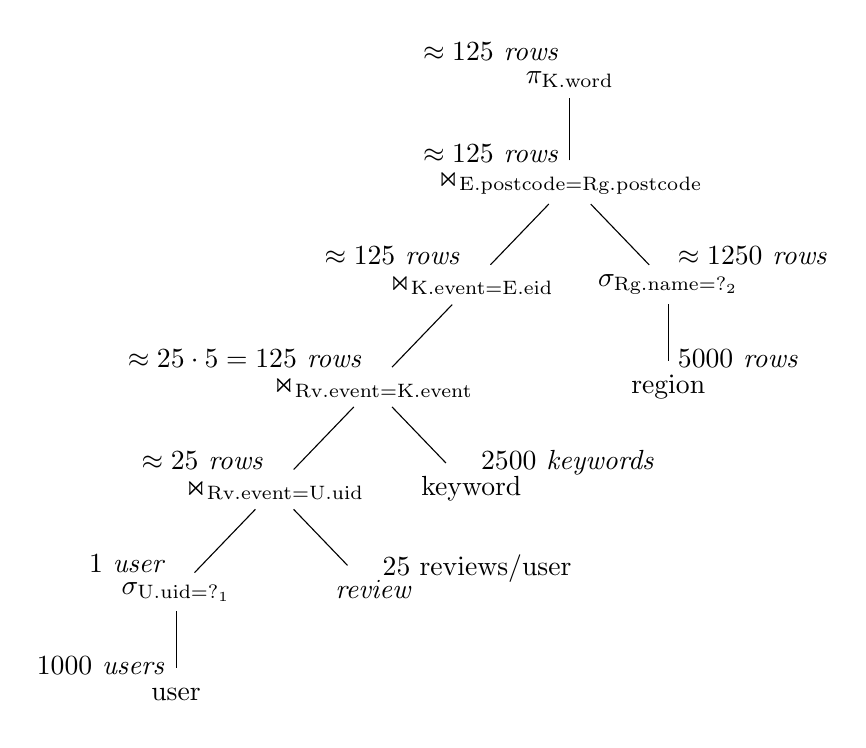
\begin{tikzpicture}[yscale = 1.3]
      \node (p) at (0, 0) {$\project_{\ra{K}{word}}$};
      \node[above left] at (p) {\strut{}\emph{$\approx 125$ rows}};
      \node (eprgp) at (0, -1) {$\njoin_{\ra{E}{postcode} = \ra{Rg}{postcode}}$} edge (p);
      \node[above left] at (eprgp) {\strut{}\emph{$\approx 125$ rows}};
      \node (keeid) at (-1.25, -2) {$\njoin_{\ra{K}{event} = \ra{E}{eid}}$} edge (eprgp);
      \node[above left] at (keeid) {\strut{}\emph{$\approx 125$ rows}};
      \node (srg) at (1.25, -2) {$\select_{\ra{Rg}{name} = ?_2}$} edge (eprgp);
      \node[above right] at (srg) {\strut{}\emph{$\approx 1250$ rows}};
      \node (rg) at (1.25, -3) {\strut{}\rel{region}} edge (srg);
      \node[above right] at (rg) {\strut{}\emph{$5000$ rows}};
      \node (rveke) at (-2.5, -3) {$\njoin_{\ra{Rv}{event} = \ra{K}{event}}$} edge (keeid);
      \node[above left] at (rveke) {\strut{}\emph{$\approx 25 \cdot 5 = 125$ rows}};
      \node (rvuuid) at (-3.75, -4) {$\njoin_{\ra{Rv}{event} = \ra{U}{uid}}$} edge (rveke);
      \node[above left] at (rvuuid) {\strut{}\emph{$\approx 25$ rows}};
      \node (k) at (-1.25, -4) {\strut{}\rel{keyword}} edge (rveke);
      \node[above right] at (k) {\strut{}\emph{$2500$ keywords}};
      \node (su) at (-5, -5) {$\select_{\ra{U}{uid} = ?_1}$} edge (rvuuid);
      \node[above left] at (su) {\strut{}\emph{$1$ user}};
      \node (rv) at (-2.5, -5) {\strut{}\emph{\rel{review}}} edge (rvuuid);
      \node[above right] at (rv) {$25$ reviews/user};
      \node (u) at (-5, -6) {\strut{}\rel{user}} edge (su);
      \node[above left] at (u) {\strut{}\emph{$1000$ users}};
    \end{tikzpicture}

    % \begin{tikzpicture}[yscale=1.2]
    %   \node (p) at (0, 0) {$\project_{\ra{E}{title}}$};
    %   \node[above right] at (p) {\strut{}\emph{$\approx 25$ rows}};
    %   \node (su) at (0, -1) {$\select_{\ra{U}{uid} = ?}$} edge (p);
    %   \node[above right] at (su) {\strut{}\emph{$\approx 25$ rows}};
    %   \node (ss) at (0, -2) {$\select_{\ra{U}{uid} = \ra{R}{user} \land \ra{E}{eid} = \ra{R}{event} \land \ra{E}{postcode} = \ra{U}{postcode}}$} edge (su);
    %   \node[above right] at (ss) {\strut{}\emph{$\approx 25000$ rows}};
    %   \node (uer) at (0, -3) {$\product$} edge (ss);
    %   \node[above left] at (uer) {\strut{}\emph{$5 \cdot 10^6 \cdot 25000 = 125 \cdot 10^9$ rows}};
    %   \node (rv) at (1, -4) {$\rel{review}$} edge (uer);
    %   \node[above right] at (rv) {\strut{}\emph{$25000$ reviews}};
    %   \node (ue) at (-1, -4) {$\product$} edge (uer);
    %   \node[above left] at (ue) {\strut{}\emph{$1000 \cdot 5000 = 5 \cdot 10^6$ rows}};
    %   \node (u) at (-2, -5) {$\rel{user}$} edge (ue);
    %   \node[above left] at (u) {\strut{}\emph{$1000$ users}};
    %   \node (e) at (0, -5) {$\rel{event}$} edge (ue);
    %   \node[above right] at (e) {\strut{}\emph{$5000$ events}};
    % \end{tikzpicture} \\

\end{enumerate}



\end{document}